\chapter{Beispielanwendung von Spark zur Datenanalyse}

Zur vertiefenden Betrachtung von Spark wird im Folgenden die Implementation einer realitätsnahen Beispielanwendung gezeigt.\\

Dazu sollen mindestens zwei verschiedene Standardbibliotheken und deren Integration in eine gemeinsame Anwendung durchgeführt werden.\\

Anschließend werden rudimentäre Skalierungs- und Stresstests der Anwendung durchgeführt und der durchgeführte Versuch unter den Kriterien \textit{Einfachheit}, \textit{Skalierbarkeit}, \textit{Erweiterbarkeit}, \textit{Robustheit}, \textit{Sicherheit} und \textit{Wartbarkeit} zusammengefasst und bewertet.

\section{Anwendungsfall}
In dem Anwendungsfall soll ein Dashboard erstellt werden, auf dem ##################
en Textnachrichten aus einem Datenstrom gelesen werden und dabei - entsprechend ihrer aktuellen Relevanz für einen Sparkbenutzer - bewertet und gefiltert werden. Als Maßstab für die Relevanz sollen Begriffen dienen, die kürzlich in der Mailingliste der Sparkbenutzer diskutiert wurden.\\

Als Datenquellen dienen einerseits die Emails aus der Malingliste\footnote{user@spark.apache.org} und andererseits der von Twitter kostenlose Datenstrom\footnote{https://dev.twitter.com/streaming/sitestreams} mit Textnachrichten (\glspl{tweet}).

\subsection{Anforderungen}

Für die Software soll folgende lose Sammlung funktionaler und nicht-funktionaler Anforderungen gelten. Mit \textit{Information} ist jeweils eine Auflistung von Twitter-Meldungen gemeint.

\begin{itemize}
	\item \textbf{A1: Zugriff auf die Information}\\
	Der Zugriff soll über eine grafische Benutzerschnittstelle erfolgen und keine Konfigurationen benötigen.
	\item \textbf{A2: Aktualität der Information}\\
	Es sollen stets Informationen dargestellt werden, die unmittelbar zuvor entstanden sind und in Quasi-Echtzeit\footnote{Eine Latenz von unter einer Minute sei hier tolerabel} verarbeitet wurden.
	\item \textbf{A3: Relevanz der Information}\\
	Die Relevanz soll an aktuellen Themen der Entwicklergemeinschaft gemessen werden.
\end{itemize}

\subsection{Hardwarekontext und Performance-Basisdaten}

Als Testumgebung dient ein \gls{cluster} aus vier identischen \gls{worker}n und einem speziellen \gls{master}knoten (Abb. \ref{figure:versuchsaufbau}).

\begin{figure}[h]
	\centering
  \includesvg[pdf]{versuchsaufbau}
	\caption{Hardwareumgebung des Programms zur Tweetanalyse}
	\label{figure:versuchsaufbau}
\end{figure}

\paragraph{Worker}
Rasperry Pi 2
\begin{itemize}
	\item CPU: 900MHz Quad-Core ARM Cortex A7
	\item RAM: 1GB SDRAM
	\item Ethernet: 100MBit/s
	\item Festspeicher: SDHC Class 4 Speicherkarte 16GB
\end{itemize}
Als Betriebssystem kommt das Debian-Derivat Raspbian\cite{raspbian} 32-Bit zum Einsatz.

\paragraph{Master}
Dell d420
\begin{itemize}
	\item CPU: 1,2 GHz Core2 Duo U2500
	\item RAM: 2GB DDR2 SDRAM
	\item Ethernet: 100MBit/s
	\item Festspeicher: 60GB 4200RPM Hard Drive
\end{itemize}
Als Betriebssystem komm Ubuntu\cite{ubuntu} 14.04 32-Bit zum Einsatz.

\paragraph{Netzwerk}
Vernetzt sind die Rechner mit \gls{rj45} über einen TP-Link TL-SF1008D Switch mit maximalem Durchsatz von 100MBit/s.

\begin{table}[ht]
	\caption{---DUMMY--- Netzwerkdurchsatz} % title of Table
	\centering % used for centering table
	\begin{tabular}{c c c c} % centered columns (4 columns)
	\hline\hline %inserts double horizontal lines
	Nachrichtengröße & Worker $\rightarrow$ Worker & Master $\rightarrow$ Worker & Worker $\rightarrow$ Master \\ [0.5ex] % inserts table
	%heading
	\hline % inserts single horizontal line
	1kB & 50ms & 837ms & 970ms \\ % inserting body of the table
	64kB & 47ms & 877ms & 230ms \\
	1MB & 31ms & 25ms & 415ms \\
	64MB & 35ms & 144ms & 2356ms \\ [1ex] 
	\hline %inserts single line
	\end{tabular}
	\label{table:nonlin} % is used to refer this table in the text
\end{table}

\subsection{Lösungsskizze}


\paragraph{Wahl des Dateisystems}

Als Quelle der persistenten Daten (Nachrichtenkorpus der Mailinglisten) kommen verschiedene Technologien in Frage:

\begin{table}[ht]
	\caption{Übersicht ausgewählter Datenquellen für Spark} % title of Table
	\centering % used for centering table
	\begin{tabular}{c c c} % centered columns (4 columns)
	\hline\hline %inserts double horizontal lines
	Name & Typ & Beschreibung\\ [0.5ex] % inserts table
	%heading
	\hline % inserts single horizontal line
	Cassandra & Datenbank & ...\\ % inserting body of the table
	HBase & Datenbank & ...\\
	HDFS & Verteiltes Dateisystem & ...\\
	Kafka & ?? & ...\\
	\hline %inserts single line
	\end{tabular}
	\label{table:dsources} % is used to refer this table in the text
\end{table}

Für diesen Versuch wird HDFS zum Verwalten der Textdatei gewählt. Für das Einlesen des Textkorpus wird keine Echtzeitfunktionalität benötigt. Weil an den Textdateien nichts geändert wird ist Versionierung ebenso unnötig wie Verknüpfungen zu anderen Datensätzen.\\

Die "`In-Memory"'-Funktionen (VERWEIS Glossar?) anderer Systeme, sind hier eher hinderlich, weil der lokale Arbeitsspeicher der Arbeitsknoten im Versuchsaufbau stark beschränkt ist und eine leicht erhöhte Latenz beim Einlesen in Kauf genommen werden kann. Das Erstellen des Feature Vektors (VERWEIS) ist nicht zeitkritisch für die Echtzeitkomponente.\\

HDFS als Komponente von Apache Hadoop ist in den Versionen 2.x deutlich bezüglich der Verfügbarkeit und Skalierbarkeit verbessert worden (VERWEIS), allerdings auch aufwändiger zu installieren. Für den Zweck dieses Versuchs wird Version 1.2.1 gewählt.

\begin{itemize}
	\item item 
	\item item
\end{itemize}

\paragraph{Wahl des Cluster-Managers}

\begin{table}[ht]
	\caption{Übersicht verfügbarer Clustermanager für Spark} % title of Table
	\centering % used for centering table
	\begin{tabular}{c c c} % centered columns (4 columns)
	\hline\hline %inserts double horizontal lines
	Name & Typ & Beschreibung\\ [0.5ex] % inserts table
	%heading
	\hline % inserts single horizontal line
	Standalone & Spezifischer Clustermanager für Spark & ...\\ % inserting body of the table
	Mesos & General Purpose & ...\\
	YARN & General Purpose & Apache Hadoop 2.x Clustermanager \\
	\hline %inserts single line
	\end{tabular}
	\label{table:cmngrs} % is used to refer this table in the text
\end{table}

Spark läuft in diesem Versuch als alleinige Computeanwendung auf dem Cluster. Es ist also nicht nötig Konkurrenz um Ressourcen zu berücksichtigen. Für diesen Versuch wird daher der Standalone Clustermanager gewählt.\\

\paragraph{Architekturübersicht}\\

Die Implementation des Anwendungsfalles soll in drei Schichten erfolgen. \\
In einer Schicht findet die Verarbeitung eingehender Emails statt und es werden die Relevanz der Begriffe bewertet (\textit{Batch Layer}).
In einer zweiten Schicht werden die Tweets aus einem Datenstrom eingelesen und deren Relevanz anhand der Bewertungen aus der ersten Schicht bewertet (\textit{Streaming Layer}).\\
In der dritten Schicht werden die als relevant eingestuften Emails in einer grafischen Oberfläche dem Benutzer zur Verfügung gestellt (\textit{Presentation Layer}).

\begin{figure}[ht!]
	\centering
  \includegraphics[scale=0.7]{data_centric_layers.pdf}
	\caption{Datenzentrierte Sicht auf die Komponenten}
	\label{figure:data_centrice_layers}
\end{figure}

\paragraph{Batch Layer}\\

\paragraph{Streaming Layer}\\

\paragraph{Presentation Layer}\\

\begin{figure}[ht!]
	\centering
  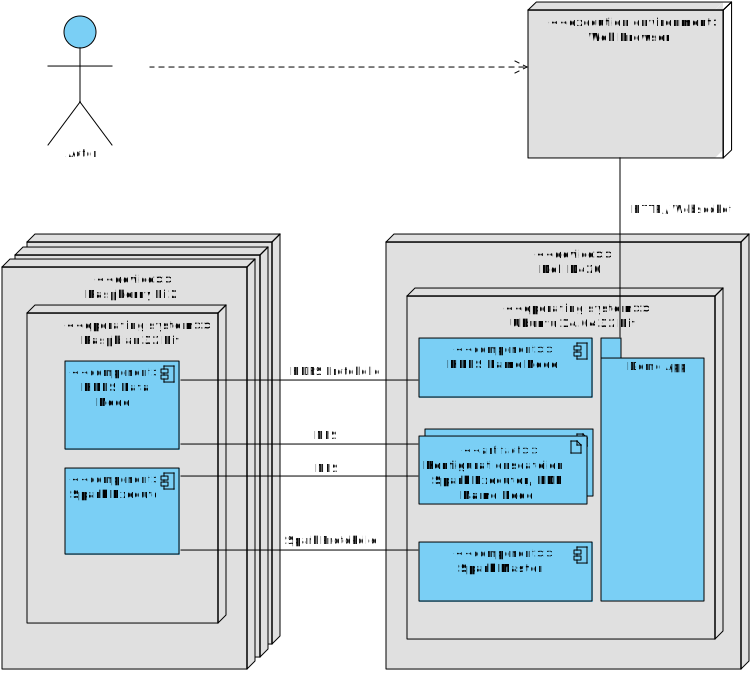
\includegraphics[scale=0.7]{demo_app_deployment.pdf}
	\caption{Verteilungssicht auf die Demo App}
	\label{figure:demo_app_verteilung}
\end{figure}


\begin{figure}[ht!]
	\centering
  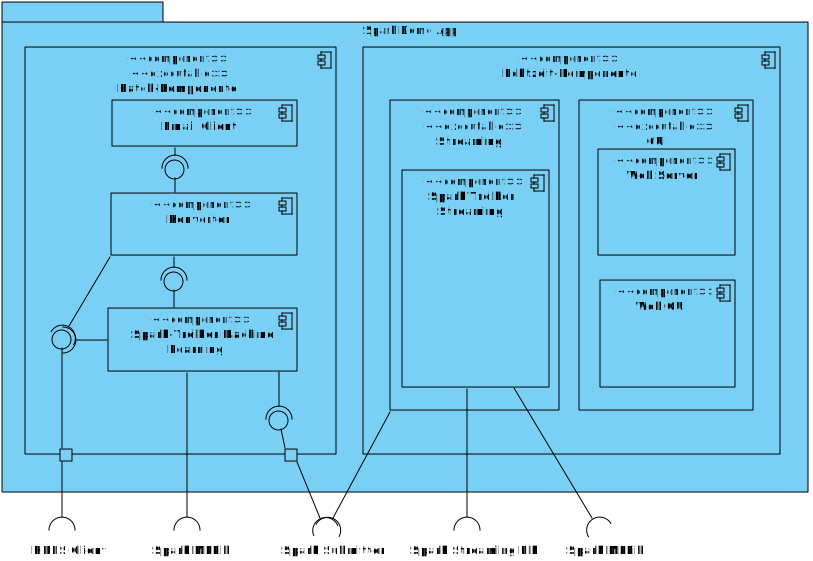
\includegraphics[scale=0.65]{demo_app_components.pdf}
	\caption{Komponentendiagramm des Demo App Packages}
	\label{figure:demo_app_komponenten}
\end{figure}

\paragraph{Batch Komponente}\\

\paragraph{Streaming-Komponente}\\

\paragraph{Presentation-Komponente}\\


\subsection{Ergebnisse und Bewertung}
\paragraph{Dashboard}
\paragraph{Laufzeitverhalten}
\paragraph{Bewertung und Probleme}


\section{Spark-basierte Implementation von Operatoren aus der Klimaforschung}
\textcolor{gray}{--- Implementation ausgewählter CDOs (sehr wenige, möglicherweise nur 1-2) mit der Core-API von Spark. Testlauf auf einem HPC Cluster mit nicht-lokalem, allerdings per Infiniband angeschlossenen Storage.
Insbesondere Betrachtung des Skalierungsverhaltens und der "`Sinnhaftigkeit"'. ---}

\subsection{Beschreibung des Problems}
\textcolor{gray}{--- Erläuterung von CDOs (Climate Data Operators). ---}
\subsection{Hardwarekontext und Performance-Basisdaten}
\textcolor{gray}{--- hier kommen die eingesetzten Systeme, und relevante Laufzeitmessungen (netzwerk, storage, cpu) hin ---}
\subsection{Architekturübersicht}
\textcolor{gray}{--- hier kommen Verteilungs- und Komponentendiagramm hin ---}
\subsection{Detailierte Lösungsbeschreibung}
\textcolor{gray}{--- hier kommen laufzeitdiagramme und codeschnipsel hin ---}
\subsection{Ergebnisse}
\textcolor{gray}{--- Tabellen und Diagramme Ergebnissen, evt. Skalierungsverhalten ---}
\textcolor{gray}{--- Bewertung ---}
